\documentclass{beamer}
\usetheme{Boadilla}

\usepackage{tikz-cd}
\usepackage{tikz}
\usepackage{mathrsfs}
\usepackage{relsize}
\usepackage{xcolor}
\usepackage{amsmath}
\usetikzlibrary{arrows.meta}
\tikzset{%
  tipA/.tip={Triangle[angle=90:6pt]},
  %tipB/.tip={Bar[sep]Square[open]}
}
\usepackage[FIGTOPCAP]{subfigure}
\usetikzlibrary{decorations.pathmorphing,backgrounds,automata}
\usepackage{graphicx}
\graphicspath{ {./Images/} }

\newtheorem{thm}{Theorem}

\usepackage{filecontents}

\begin{filecontents}{\jobname.bib}
@TECHREPORT{RePEc:cwl:cwldpp:159,
    title = {Commercial Banks as Creators of 'Money'},
    author = {Tobin, James},
    year = {1963},
    institution = {Cowles Foundation for Research in Economics, Yale University},
    type = {Cowles Foundation Discussion Papers},
    number = {159},
    url = {http://EconPapers.repec.org/RePEc:cwl:cwldpp:159}
}
\end{filecontents}

\title{State Stabilization in Open Quantum Systems}
%\subtitle{and Applications}
\author{David Campbell}
\institute{UMass Lowell}
\date{May 3, 2019}



\begin{document}

\begin{frame}
\titlepage
\end{frame}

\begin{frame}
\frametitle{ Quantum Information Science }

\begin{itemize}

\item Computation power needs to keep up with the explosive increase in data/information.
\item Discovery of quantum algorithms that can factor large integers (Shor's Algorithm).
\item Quantum Simulation - molecules are computational complex.
\item Quantum teleportation - we can transmit quantum information when sender and receiver share an entanglement.

\end{itemize}

\end{frame}

\begin{frame}
\frametitle{Decoherence of a ``Cat"}
\begin{columns}
\begin{column}{0.47\textwidth}
 Real Part
 $\rho(x,x') = \langle x | \rho | x' \rangle $
 \includegraphics[scale=.3]{cat_state.pdf}
 \end{column}
 \begin{column}{0.47\textwidth}
 ``Cat" State
\begin{equation}
| \Psi \rangle \propto | \alpha \rangle + | - \alpha \rangle \nonumber
\end{equation}
\par
\vspace{.75in}
After decoherence
\begin{equation}
\rho \propto | \alpha \rangle \langle \alpha | + | - \alpha \rangle \langle - \alpha |  \nonumber 
\end{equation}
%% \includegraphics[scale=1]{cat_state.pdf}
 \end{column}
\end{columns}
%\footcite{RePEc:cwl:cwldpp:159}
\end{frame}

\begin{frame}
\frametitle{Outline}
\tableofcontents
\section{Open Quantum System Formalism}
\section{Dark States}
\section{Adiabatic Elimination}
\section{Bell State Stabilization}
\subsection{Symmetric}
\subsection{Chiral}
\section{Four-Qubit Entanglement}

\end{frame}


\begin{frame}{The columns environment}
\frametitle{Open Quantum System Framework}
\begin{columns}
    \begin{column}{0.47\textwidth}
      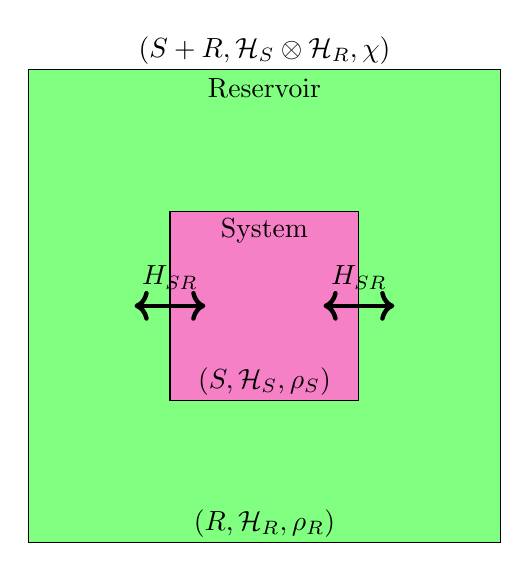
\begin{tikzpicture}[scale=.60]
	\draw [fill=green!50] (10,10) -- (0,10) -- (0,0) -- (10,0)--(10,10);
	\node at (5,10.4) {\scalebox{1.0}{$\left(S+R, \mathcal{H}_S \otimes \mathcal{H}_R, \chi \right)$}} ;
	\draw [fill=magenta!50] (7,7) rectangle (3,3 );
	\node at (5,.4) { \scalebox{1.0}{\textcolor{black}{$\left(R, \mathcal{H}_R, \rho_R \right)$}} };
	\node at (5,3.4) {\scalebox{1.0}{$\left(S, \mathcal{H}_S, \rho_S \right)$}};
	\draw[ultra thick, <->] (2.25,5) -- (3.75,5);
	\draw[ultra thick, <->] (6.25,5) -- (7.75,5);
	\node at (3,5.6) {\scalebox{1.0}{$H_{SR}$}};
	\node at (7,5.6) {\scalebox{1.0}{$H_{SR}$}};
	\node at (5,6.6) {\scalebox{1.0}{System}};
	\node at (5,9.6) {\scalebox{1.0}{Reservoir}};
	\end{tikzpicture}
    \end{column}
    
    \begin{column}{0.43\textwidth}
       
        \begin{equation}
   		\dot{\chi} = - \frac{i}{\hbar} [H , \chi] \nonumber 
        \end{equation}
        \begin{equation}
       \chi = \sum_n p_n | \Psi_n \rangle \langle \Psi_n | \nonumber 
        \end{equation}
        \begin{equation}
        H = H_S + H_R + H_{SR} \nonumber 
        \end{equation}
        Born Approximation
        \begin{equation}
\tilde{\chi}(t) = \tilde{\rho}_{\mathcal{S}}(t) \otimes \rho_{\mathcal{R}} \nonumber 
\end{equation}
Markov Approximation
\begin{equation}
\left\langle b_\alpha^{\dagger}(t) b_\alpha(s) \right\rangle \sim \delta(t-s) \nonumber
\end{equation}
    \end{column}
    
\end{columns}
\end{frame}

\begin{frame}
\frametitle{Example: Driven-Qubit coupled to Thermal Reservoir}

\begin{equation}
\frac{H}{\hbar}  = \sum_n \omega_{cn} b_n^\dagger b_n + \frac{\epsilon}{2} \sigma_z + \Omega \cos( \omega_l t )\sigma_x + g \sigma_{x} \otimes\sum_n \left[ b_n + b_n^\dagger \right] \nonumber 
\end{equation}
\centering
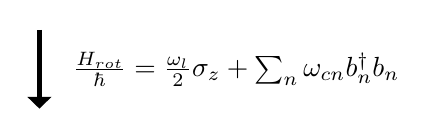
\begin{tikzpicture}
\draw[ultra thick , -tipA] (0,0)--(0,-1);
\node at (2.5,-0.5) {\scalebox{1.0}{$\frac{H_{rot}}{\hbar} = \frac{\omega_l}{2}\sigma_z + 
\sum_n \omega_{cn}  b_n^\dagger b_n$}} ;
\end{tikzpicture}


\begin{equation}
\frac{H'}{\hbar}  \approx  \frac{\delta}{2} \sigma_z +\frac{ \Omega}{2} \sigma_x + \boxed{ \underbrace{ g   \sum_n \sigma  b_n^\dagger +g^* \sum_n \sigma^\dagger b_n}_{=  \frac{H_{SR}}{\hbar}  }} \nonumber
\end{equation}

Post rotating-wave approximation, we get a Jaynes-Cummings interaction.

\end{frame}



\begin{frame}
\frametitle{Example: Driven-Qubit coupled to Thermal Reservoir}

\begin{align}\label{Optical Block ME}
\dot{\rho}_{\mathcal{S}} & =  - i \frac{\delta}{2} [ \sigma_z, \rho ] - i \frac{\Omega}{2} [ \sigma_x , \rho ] + \gamma ( 1 + N_{\omega_b} ) \left( \sigma \rho_{\mathcal{S}} \sigma^\dagger - \frac{1}{2} \left\lbrace \sigma^\dagger \sigma , \rho_{\mathcal{S}} \right\rbrace \right)  \nonumber \\
& \quad + \gamma N_{\omega_b} \left( \sigma^\dagger \rho_{\mathcal{S}} \sigma - \frac{1}{2} \left\lbrace \sigma \sigma^\dagger , \rho_{\mathcal{S}} \right\rbrace \right) \nonumber
\end{align}

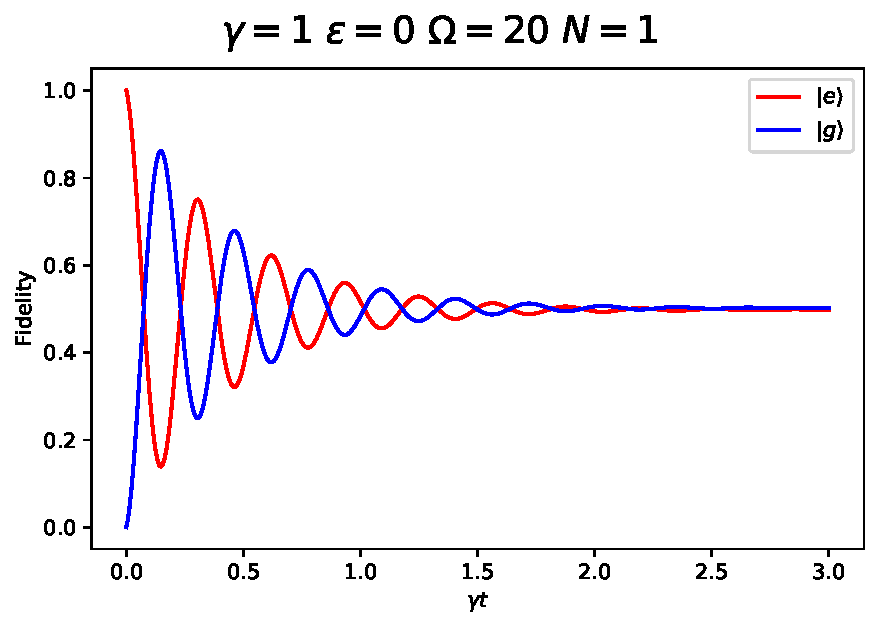
\includegraphics[scale=.5]{decoherence.pdf}

\end{frame}

\begin{frame}
\frametitle{Liouvillian}
\begin{equation}
\dot{\rho} = \mathcal{L} \rho \nonumber
\end{equation}
\begin{equation}\label{Liovuillian}
\mathcal{L}\bullet = - \frac{i}{\hbar} [ H , \bullet ] + \sum_n \gamma_l \left( c_l \bullet c_l^\dagger - \frac{1}{2} \left\lbrace c_l^\dagger c_l , \bullet \right\rbrace \right)\nonumber
\end{equation}
\begin{equation}
\mathcal{D}[c_l] \rho = \left( c_l \rho c_l^\dagger - \frac{1}{2} \left\lbrace c_l^\dagger c_l , \rho \right\rbrace \right) \nonumber 
\end{equation}
\begin{equation}
\rho(t) = e^{\mathcal{L}t} \rho = \rho_{ss} +  \sum_n e^{\lambda_n} \rho_n \nonumber
\end{equation}
We use fidelity to measure ``closeness" of the steady state, $\rho_{ss}$, to another, $|\Phi \rangle$, which is frequently entangled.
\begin{equation}
F_{| \Phi \rangle} = tr \lbrace | \Phi \rangle \langle \Phi |  \rho_{ss} \rbrace \nonumber
\end{equation}
Rate of stabilization is called the ``gap"
\begin{equation}
\Delta_{\mathcal{L}} = \min\{Re[\lambda_{n}]\}
\end{equation}
\end{frame}

\begin{frame}
\frametitle{Dark States}

\begin{thm}\label{Theorem}
A pure state is stabilized, $\mathcal{L}\left( |\Phi \rangle \langle \Phi |  \right)=0$, if and only if the following two conditions are satisfied: 

(1) $H' | \Phi \rangle = \Im( \lambda )| \Phi \rangle$ for some $\lambda \in \mathbb{C}$

(2) $c_l' | \Phi \rangle = 0$ for some $\lambda_l \in \mathbb{C}$ with $\sum_l g_l |\lambda_l|^ 2 = Re ( \lambda ) $.

When pure steady steady state meets these conditions it is called a \textbf{dark state}.

\end{thm}

$H' = H - i \sum_l g_l \lambda_l (c_l')^\dagger + i \sum g_l \lambda_l^* c_l'$

$c_l' = c_l - \lambda_l$


\end{frame}



\begin{frame}
\frametitle{Adiabatic Elimination Problem}


\begin{columns}

\begin{column}{0.47\textwidth}
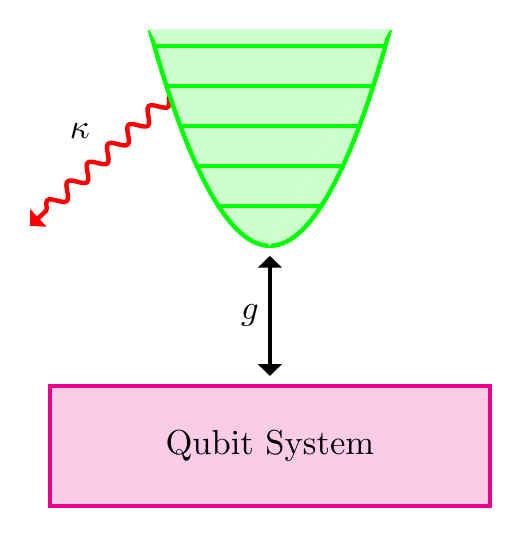
\begin{tikzpicture}[x=1.0in,y=1.0in]
\draw [red, ultra thick,-tipA,decorate,decoration={snake,post length=1.65mm}] (-.5,.75) -- (-1.2, .1);
\node at (-.95,.575) {\scalebox{1.25}{$\kappa$}} ;
\filldraw[color=green!100, fill=green!20 , ultra thick] (0,0) parabola (0.6,1.08) ;
\filldraw[color=green!100, fill=green!20 , ultra thick] (0.0,0.0) parabola (-0.6,1.08) ;
\filldraw[color=green!20, fill=green!20] (0,0) -- ( -0.6,1.08) -- ( 0.6,1.08);
\draw[color=green!100 , ultra thick] (-0.36514837167011072,.4) -- (0.36514837167011072,.4);
\draw[color=green!100 , ultra thick] (0.2581988897471611,.2) -- (-0.2581988897471611,.2);
\draw[color=green!100 , ultra thick] (0.44721359549995793,.6) -- (-0.44721359549995793,.6);
\draw[color=green!100 , ultra thick] (0.5163977794943222,.8) -- (-0.5163977794943222,.8);
\draw[color=green!100 , ultra thick] (0.57735026918962573,1.0) -- (-0.57735026918962573,1.0);
\filldraw[color=magenta!100, fill=magenta!20, ultra thick] (-1.1 ,-1.3 ) rectangle (1.1, -.7);
\node at (0,-1.0) {\scalebox{1.25}{Qubit System}} ;
\draw[black, ultra thick , tipA-tipA] (0.0,-0.65) -- (0.0,-0.05);
\node at (-.1, -.35) {\scalebox{1.25}{$g$}} ;
\end{tikzpicture}
\end{column}

\begin{column}{0.47\textwidth}
Quasi-static bath (low Q-value)
\begin{equation}\label{ansatz}
\chi \approx \rho_S(t) \otimes | 0 \rangle \langle 0 | \nonumber
\end{equation}
``Engineered" a coupling between a qubit system and a harmonic oscillator to facilitate entanglement stabilization.
\begin{eqnarray}\label{D_AB}
\frac{H_R}{\hbar} & = & \Delta b^{\dagger} b \nonumber \\
\frac{H_{SR}}{\hbar} & = & g \left( b^{\dagger} \hat{S} e^{i \phi } + b \hat{S}^{\dagger} e^{-i \phi} \right) \nonumber
\end{eqnarray}

\end{column}

\end{columns}

\end{frame}

\begin{frame}
\frametitle{Adiabatic Elimination Problem}

%Decay of the cavity causes an effective or ``engineered" decay on qubits determined through adiabatic elimination. 
%\vspace{3mm}

Quasi-static bath (low Q-value)
\begin{equation}\label{ansatz}
\chi \approx \rho_S(t) \otimes | 0 \rangle \langle 0 | \nonumber
\end{equation}

Coupled weekly, $\kappa \gg g$, to a \textbf{single} harmonic oscillator
\begin{eqnarray}\label{D_AB}
\frac{H_R}{\hbar} & = & \Delta b^{\dagger} b \nonumber \\
\frac{H_{SR}}{\hbar} & = & g \left( b^{\dagger} \hat{S} e^{i \phi } + b \hat{S}^{\dagger} e^{-i \phi} \right). 
\end{eqnarray}
The equation of motion of the full system+reservior is
\begin{equation}
\dot{\chi} = - \frac{i}{\hbar} [H , \chi] + \kappa \mathcal{D}[a]\chi.
\end{equation}

\end{frame}



\begin{frame}
\frametitle{Adiabatic Elimination Problem}
Construct a perturbative solution and trace of the reservoir
\begin{equation}
\dot{\tilde{\rho}}_S =   \int_0^t d\tau \; tr_R \left\lbrace \left[ \tilde{H}_{SR}(t) , \left[ \tilde{H}_{SR}(\tau), \tilde{\rho}_S(t) \otimes | 0 \rangle_R \langle 0 | \right] \right]  \right\rbrace. \nonumber 
\end{equation}
Evaluating the partial trace
\begin{align}\label{decay expodential}
tr_R \lbrace \mathcal{\tilde{L}}_{SR}(t) \mathcal{\tilde{L}}_{SR}(\tau) \tilde{\chi} \rbrace & =  g^2 e^{ - \kappa ( t - \tau )/ 2 } \lbrace \mathcal{S}_1'^{\dagger}(t) \mathcal{S}_1'(\tau) \nonumber \\
& \quad +  \mathcal{S}_1'(t) \mathcal{S}_1'^{\dagger}(\tau) - \mathcal{S}_2'^{\dagger}(t) \mathcal{S}_1'^{\dagger}(\tau) - \mathcal{S}_2'(t) \mathcal{S}_1'(t) \rbrace \tilde{\rho}_S(t). \nonumber 
\end{align}
Make the Markov approximation $e^{ - \kappa ( t - \tau ) / 2} \rightarrow  2 \delta( t - \tau ) / \kappa$ and $t \rightarrow \tau$. The punchline is,
\begin{eqnarray} \label{Engineered Reduced System}
 \dot{\rho}_S  =  - \frac{i}{\hbar} [H_S, \rho_S] + \frac{4 g^2}{\kappa} \mathcal{D}[\hat{S}] \rho_S. \nonumber
\end{eqnarray}
%$\hat{S}$ is our ``engineered" jump operator. And $\Gamma = \frac{4 g^2}{\kappa}$ is our engineered dissipation rate
\end{frame}

\begin{frame}
\frametitle{Symmetric Scheme}
\begin{columns}

   \begin{column}{0.43\textwidth}
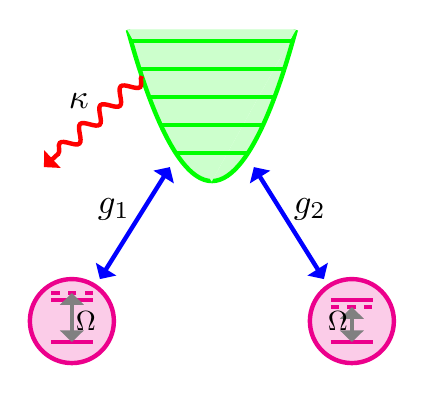
\begin{tikzpicture}[x=.7in,y=.7in]
\filldraw[color=green!100, fill=green!20 , ultra thick] (0,0) parabola (0.6,1.08) ;
\filldraw[color=green!100, fill=green!20 , ultra thick] (0.0,0.0) parabola (-0.6,1.08) ;
\filldraw[color= magenta!100, fill=magenta!20, ultra thick](-1,-1) circle (.3);
\filldraw[color=magenta!100, fill=magenta!20, ultra thick](1,-1) circle (.3);
\filldraw[color=green!20, fill=green!20] (0,0) -- ( -0.6,1.08) -- ( 0.6,1.08);
\draw[blue, ultra thick , tipA-tipA] (-0.8,-.7) -- (-0.3,0.1);
\draw[blue, ultra thick , tipA-tipA] (0.8,-.7) -- (0.3,0.1);
\draw [red, ultra thick,-tipA,decorate,decoration={snake,post length=1.65mm}] (-.5,.75) -- (-1.2, .1);
\node at (-.95,.575) {\scalebox{1.25}{$\kappa$}} ;
\draw[color= magenta!100 , ultra thick] (-.85,-1.15)--(-1.15,-1.15);
\draw[color= magenta!100 , ultra thick] (-.85,-.85)--(-1.15,-0.85);
\draw[color= magenta!100 , ultra thick] (.85,-1.15)--(1.15,-1.15);
\draw[color= magenta!100 , ultra thick] (.85,-.85)--(1.15,-0.85);
\draw [dashed,color= magenta!100 , ultra thick] (.85,-.90)--(1.15,-0.90);
\draw [dashed,color= magenta!100 , ultra thick] (-.85,-.80)--(-1.15,-0.80);
\draw [gray, ultra thick , tipA-tipA] (-1.0,-1.15)--(-1.0,-.8);
\draw [gray, ultra thick , tipA-tipA] (1.0,-1.15)--(1.0,-.9);
\node at (-0.9,-1.0) {\scalebox{1.0}{$\Omega$}} ;
\node at (0.9,-1.0) {\scalebox{1.0}{$\Omega$}} ;
%\node at (-1.37,-0.85) {\scalebox{1.0}{$+\delta$}} ;
%\node at (1.37,-0.85) {\scalebox{1.0}{$-\delta$}} ;
\draw[color=green!100 , ultra thick] (-0.36514837167011072,.4) -- (0.36514837167011072,.4);
\draw[color=green!100 , ultra thick] (0.2581988897471611,.2) -- (-0.2581988897471611,.2);
\draw[color=green!100 , ultra thick] (0.44721359549995793,.6) -- (-0.44721359549995793,.6);
\draw[color=green!100 , ultra thick] (0.5163977794943222,.8) -- (-0.5163977794943222,.8);
\draw[color=green!100 , ultra thick] (0.57735026918962573,1.0) -- (-0.57735026918962573,1.0);
\node at (.7, -.2) {\scalebox{1.25}{$g_2$}} ;
\node at (-.7, -.2) {\scalebox{1.25}{$g_1$}} ;
\end{tikzpicture}   
   
\end{column}

   \begin{column}{0.43\textwidth}
\begin{eqnarray}\label{Two_Qubit_Hamiltonian}
\frac{H'_R}{\hbar} & = & 0 \nonumber \\
\frac{H'_S}{\hbar} & \approx & \sum_{i=1}^2 \left( \frac{\delta_i}{2}  \sigma_{zi}  + \frac{\Omega_i}{2} \sigma_{x1} \right) \nonumber \\
\frac{H'_{SR}}{\hbar} & \approx &  b^\dagger \underbrace{( g_1 \sigma_1 + g_2 \sigma_2 )}_\text{$=g\hat{S}$} + h.c.  \nonumber 
\end{eqnarray} 

\end{column}

\end{columns}
\vspace{.5cm}
\centering
Choose homogeneous couplings $g_1 = g_2 =g $.
\begin{equation}
\boxed{\dot{\rho}_S = - \frac{i}{\hbar} [H_S' , \rho_S ] + \frac{4g^2}{\kappa}\mathcal{D}[ \sigma_1 + \sigma_2 ] \rho_S} \nonumber
\end{equation}
\end{frame}

\begin{frame}
\frametitle{Dissipative Interaction}
\begin{align}\label{Expand reduced system ME}
\dot{\rho}_S  & = - \frac{i}{\hbar} [H'_S, \rho_S]  +  \frac{4g^2}{\kappa}\mathcal{D}[\sigma_1]\rho_S +  \frac{4g^2}{\kappa} \mathcal{D}[\sigma_2]\rho_S \nonumber \\
& \quad +\textcolor{blue}{  \frac{4g^2}{\kappa} \bigg[  \left(\sigma_1 \rho_S \sigma_2^\dagger - \frac{1}{2} \left \lbrace \sigma_2^\dagger \sigma_1 , \rho_S \right\rbrace \right) + \left( \sigma_2 \rho_S \sigma_1^\dagger - \frac{1}{2} \left \lbrace \sigma_1^\dagger \sigma_2 , \rho_S \right\rbrace \right) \biggr]} \nonumber
\end{align}
\centering
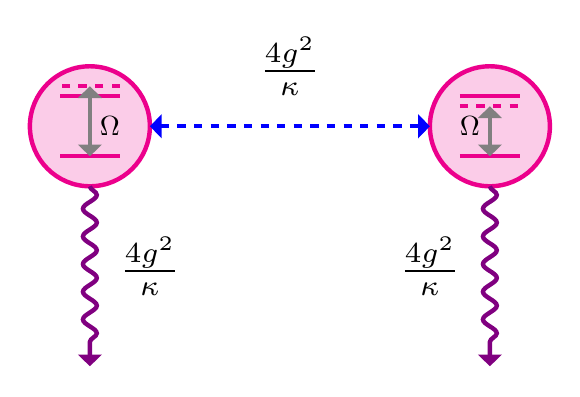
\begin{tikzpicture}[x=1.0in,y=1.0in]
\filldraw[color= magenta!100, fill=magenta!20, ultra thick](-.6,-1) circle (.3);
\filldraw[color=magenta!100, fill=magenta!20, ultra thick](1.4,-1) circle (.3);
\draw[color= magenta!100 , ultra thick] (-.45,-1.15)--(-0.75,-1.15);
\draw[color= magenta!100 , ultra thick] (-.45,-.85)--(-0.75,-0.85);
\draw[color= magenta!100 , ultra thick] (1.25,-1.15)--(1.55,-1.15);
\draw[color= magenta!100 , ultra thick] (1.25,-.85)--(1.55,-0.85);
\draw[blue , ultra thick , dashed , tipA-tipA] (-.3, -1.0) --(1.1,-1.0);
%\draw[orange , ultra thick , dashed , tipA-] (-.3, -1.15) --(1.1,-1.15);
\draw[violet , ultra thick , -tipA , decorate , decoration={snake,post length=1.65mm}] (-.6, -1.3) --(-.6,-2.2);
\draw[violet , ultra thick , -tipA , decorate , decoration={snake,post length=1.65mm}] (1.4, -1.3) --(1.4,-2.2);
\node at (-0.5,-1.0) {\scalebox{1.0}{$\Omega$}} ;
\node at (1.3,-1.0) {\scalebox{1.0}{$\Omega$}} ;
%\node at (-0.97,-0.85) {\scalebox{1.0}{$+\delta$}} ;
%\node at (1.77,-0.85) {\scalebox{1.0}{$-\delta$}} ;
\draw [gray, ultra thick , tipA-tipA] (-0.6,-1.15)--(-0.6,-.8);
\draw [gray, ultra thick , tipA-tipA] (1.4,-1.15)--(1.4,-.9);
\draw [dashed,color= magenta!100 , ultra thick] (1.25,-.90)--(1.55,-0.90);
\draw [dashed,color= magenta!100 , ultra thick] (-.45,-.80)--(-0.75,-0.80);
\node at (0.4,-.7) {\scalebox{1.5}{$\frac{4 g^2 }{\kappa}$}} ;
\node at (-0.3,-1.7) {\scalebox{1.5}{$\frac{4 g^2}{\kappa}$}} ;
\node at (1.1,-1.7) {\scalebox{1.5}{$\frac{4 g^2}{\kappa}$}} ;
\end{tikzpicture}

\end{frame}

\begin{frame}
\frametitle{Dark States (Symmetric Case)}
\begin{columns}

\begin{column}{0.47\textwidth}
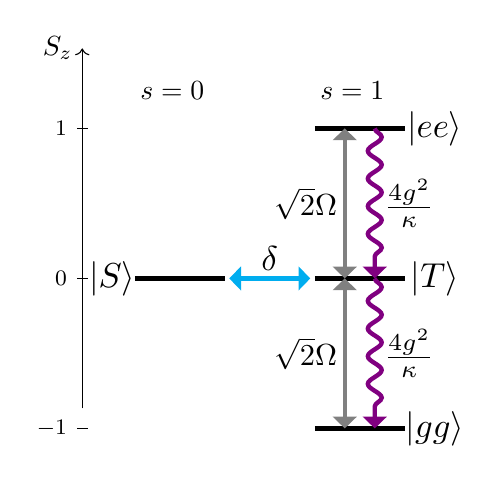
\begin{tikzpicture}[x=.75in,y=.75in]
%\begin{scope}[shift={(-1.0in,0.0in)}]
\draw[ultra thick] (0.3,0.0) -- (0.90,0.0);
\draw[ultra thick] (1.5,-1.0) -- (2.1,-1.0);
\draw[ultra thick] (1.5,0.0) -- (2.1,0.0);
\draw[ultra thick] (1.5,1.0) -- (2.1,1.0);
\node at (0.15,0.0) {\scalebox{1.25}{$\left| S \right\rangle$}} ;
\node at (2.30,-1.0) {\scalebox{1.25}{$\left| gg \right\rangle$}} ;
\node at (2.30,0.0) {\scalebox{1.25}{$\left| T \right\rangle$}} ;
\node at (2.30,1.0) {\scalebox{1.25}{$\left| ee \right\rangle$}} ;
\node at (1.44,-.5) {\scalebox{1.1}{$\sqrt{2} \Omega$}} ;
\node at (1.44,0.5) {\scalebox{1.1}{$\sqrt{2} \Omega$}} ;
\node at (2.13,-.5) {\scalebox{1.25}{$\frac{4g^2}{\kappa}$}} ;
\node at (2.13,.5) {\scalebox{1.25}{$\frac{4g^2}{\kappa}$}} ;
%\node at (6.0,3.0) {\scalebox{1.0}{$\frac{8g^2}{\kappa}$}} ;
%\node at (6.0,1.0) {\scalebox{1.0}{$\frac{8g^2}{\kappa}$}} ;
\draw[cyan, ultra thick , tipA-tipA] (.93,0) -- (1.47,0);
\node at (1.2, 0.13) {\scalebox{1.25}{$ \delta $}};
\draw[gray, ultra thick , tipA-tipA] (1.7,-1) -- (1.7,0);
\draw[gray, ultra thick , tipA-tipA] (1.7,0) -- (1.7,1);
%\draw[gray, ultra thick , tipA-tipA] (4.6,2) -- (4.6,4);
%%\draw[red, ultra thick, tipA-,decorate, decoration={ snake , post length=2mm }  ] (5.4,0) -- (5.4,2);
%%\draw[red, ultra thick, tipA-,decorate, decoration={snake}] (5.4,2) -- (5.4,4);
%\draw [red, ultra thick,-tipA,decorate,decoration={snake,post length=1.65mm}] (5.4,4) -- (5.4,2);
\draw [violet, ultra thick,-tipA,decorate,decoration={snake,post length=1.65mm}] (1.9,0) -- (1.9,-1);
\draw [violet, ultra thick,-tipA,decorate,decoration={snake,post length=1.65mm}] (1.9,1) -- (1.9,0);
\node at (0.55,1.25) {\scalebox{1.0}{$s=0$}} ;
\node at (1.75,1.25) {\scalebox{1.0}{$s=1$}} ;
\draw[->,yshift=1.0in] (-0.05,-2.2) -- (-.05,0.2) node[left] {$S_z$};
\foreach \y in {-1,0,1} \draw[shift={(-0.05,\y)}] (2pt,0pt) --(-2pt,0pt) node[left] {\footnotesize $\y$};
%\end{scope}
\end{tikzpicture}
\end{column}

 \begin{column}{0.47\textwidth}
We consider the eigenvalue problem form \textbf{Theorem 1} for our engineered jump operator, $\hat{S} = \sigma_1 + \sigma_2$
 \begin{equation}
 | \Phi \rangle = \frac{1}{\sqrt{1 + | \alpha |^2}} ( |gg \rangle + \alpha |S\rangle)
 \end{equation}
 
\end{column}

\end{columns}

\end{frame}

\begin{frame}
\centering 
\frametitle{ Bell State Stabilization (Symmetric Case)}
  $ |\Phi \rangle \propto |gg\rangle + \alpha | S \rangle  \quad H_S'| \Phi \rangle = 0 \Longrightarrow \alpha = \frac{\Omega}{\sqrt{2} \delta }$
  
\vspace{3mm}  
  
  $\delta_1 = - \delta_2 = \delta$

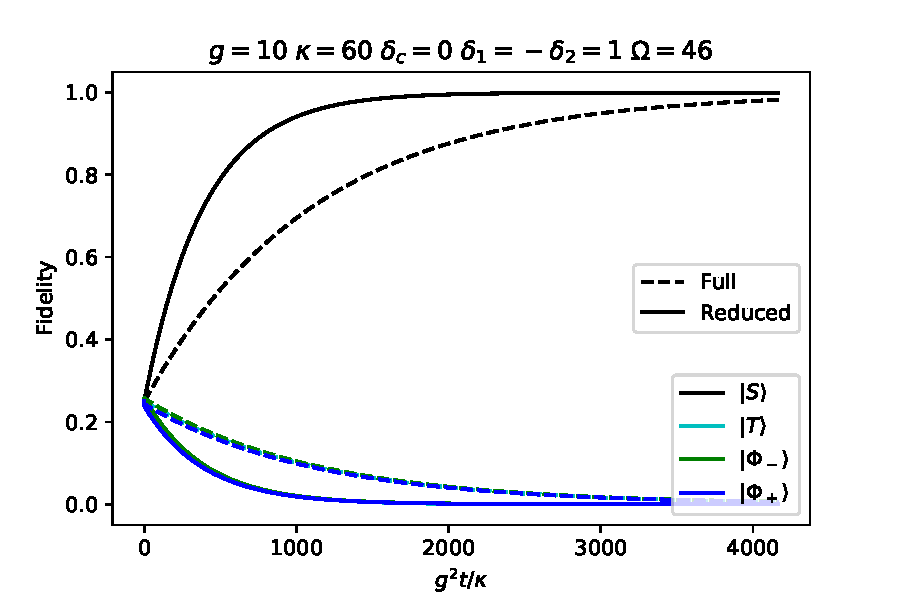
\includegraphics[scale=.6]{Sym_stabilization.pdf}

\end{frame}


\begin{frame}
\frametitle{Performance Metric}
We define a new performance metric:
$M = F_{| S \rangle } \Delta_{\mathcal{L}}/\Gamma$ with $\Gamma = \frac{4g^2}{\kappa}$.

\centering

\vspace{3mm}

%$ \dot{P}_{| S \rangle } = \langle S | \mathcal{L} \rho_S | S \rangle$
$  \dot{P}_{|S\rangle} = \Gamma_{|ee\rangle}P_{|ee \rangle} + \Gamma_{|S\rangle} P_{|S\rangle} + \Gamma_{|T\rangle} P_{|T\rangle} + \Gamma_{|ee \rangle} P_{|ee\rangle} $

\vspace{3mm}

$\Delta_\mathcal{L} \approx \Gamma_{|gg\rangle} \quad  F_{|S\rangle }= \frac{|\alpha|^2|}{1 + |\alpha|^2} $

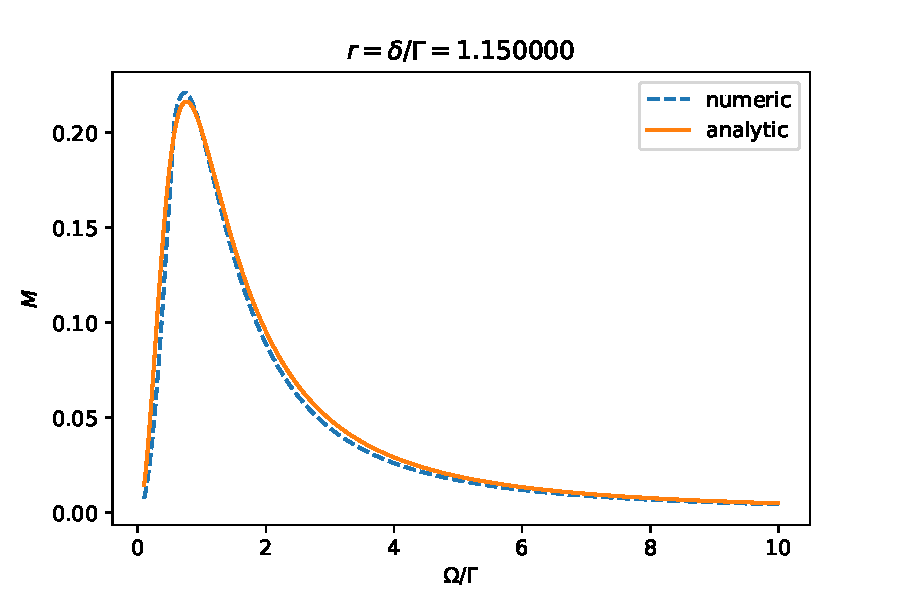
\includegraphics[scale=.5]{Sym_Anal_Num.pdf}
\end{frame}

\begin{frame}
\frametitle{Chiral Case}
Addition of qubit-qubit couplings.
\begin{eqnarray}
\frac{H'_S}{\hbar} & = & \sum_{i=1}^2 \left( \frac{\delta_i}{2}  \sigma_{zi}  + \frac{\Omega_i}{2} \sigma_{x1} \right) + \textcolor{teal}{J \sigma_1 \sigma_2^\dagger + J^* \sigma_1^\dagger \sigma_2} \nonumber 
\end{eqnarray} 

\begin{columns}

 \begin{column}{0.47\textwidth}
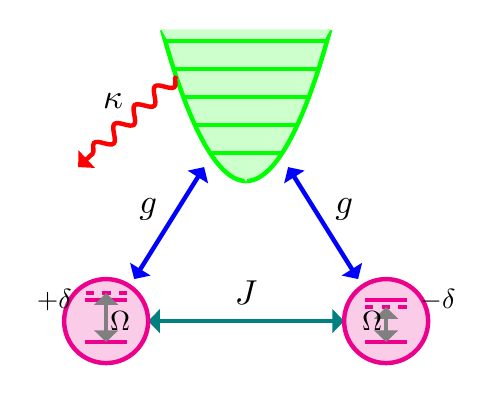
\begin{tikzpicture}[x=.7in,y=.7in]
\filldraw[color=green!100, fill=green!20 , ultra thick] (0,0) parabola (0.6,1.08) ;
\filldraw[color=green!100, fill=green!20 , ultra thick] (0.0,0.0) parabola (-0.6,1.08) ;
\draw[teal , ultra thick , tipA-tipA] (-.7, -1) -- (.7, -1) ;
\node at (0, -0.8) {\scalebox{1.25}{$J$}} ;
\filldraw[color= magenta!100, fill=magenta!20, ultra thick](-1,-1) circle (.3);
\filldraw[color=magenta!100, fill=magenta!20, ultra thick](1,-1) circle (.3);
\filldraw[color=green!20, fill=green!20] (0,0) -- ( -0.6,1.08) -- ( 0.6,1.08);
\draw[blue, ultra thick , tipA-tipA] (-0.8,-.7) -- (-0.3,0.1);
\draw[blue, ultra thick , tipA-tipA] (0.8,-.7) -- (0.3,0.1);
\node at (.7, -.2) {\scalebox{1.25}{$g$}} ;
\node at (-.7, -.2) {\scalebox{1.25}{$g$}} ;
\node at (-.95,.575) {\scalebox{1.25}{$\kappa$}} ;
\draw [red, ultra thick,-tipA,decorate,decoration={snake,post length=1.65mm}] (-.5,.75) -- (-1.2, .1);
\draw[color= magenta!100 , ultra thick] (-.85,-1.15)--(-1.15,-1.15);
\draw[color= magenta!100 , ultra thick] (-.85,-.85)--(-1.15,-0.85);
\draw[color= magenta!100 , ultra thick] (.85,-1.15)--(1.15,-1.15);
\draw[color= magenta!100 , ultra thick] (.85,-.85)--(1.15,-0.85);
\draw [dashed,color= magenta!100 , ultra thick] (.85,-.90)--(1.15,-0.90);
\draw [dashed,color= magenta!100 , ultra thick] (-.85,-.80)--(-1.15,-0.80);
\draw [gray, ultra thick , tipA-tipA] (-1.0,-1.15)--(-1.0,-.8);
\draw [gray, ultra thick , tipA-tipA] (1.0,-1.15)--(1.0,-.9);
\node at (-0.9,-1.0) {\scalebox{1.0}{$\Omega$}} ;
\node at (0.9,-1.0) {\scalebox{1.0}{$\Omega$}} ;
\node at (-1.37,-0.85) {\scalebox{1.0}{$+\delta$}} ;
\node at (1.37,-0.85) {\scalebox{1.0}{$-\delta$}} ;
\draw[color=green!100 , ultra thick] (-0.36514837167011072,.4) -- (0.36514837167011072,.4);
\draw[color=green!100 , ultra thick] (0.2581988897471611,.2) -- (-0.2581988897471611,.2);
\draw[color=green!100 , ultra thick] (0.44721359549995793,.6) -- (-0.44721359549995793,.6);
\draw[color=green!100 , ultra thick] (0.5163977794943222,.8) -- (-0.5163977794943222,.8);
\draw[color=green!100 , ultra thick] (0.57735026918962573,1.0) -- (-0.57735026918962573,1.0);
\end{tikzpicture}
\end{column}
%
\begin{column}{0.47\textwidth}
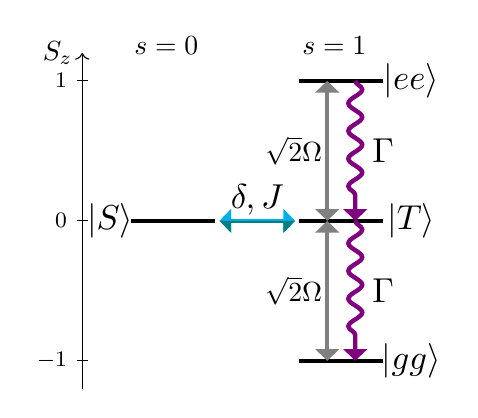
\begin{tikzpicture}[x=0.7in,y=0.7in]
\draw[ultra thick] (0.3,0.0) -- (0.90,0.0);
\draw[ultra thick] (1.5,-1.0) -- (2.1,-1.0);
\draw[ultra thick] (1.5,0.0) -- (2.1,0.0);
\draw[ultra thick] (1.5,1.0) -- (2.1,1.0);
\node at (0.15,0.0) {\scalebox{1.25}{$\left| S \right\rangle$}} ;
\node at (2.30,-1.0) {\scalebox{1.25}{$\left| gg \right\rangle$}} ;
\node at (2.30,0.0) {\scalebox{1.25}{$\left| T \right\rangle$}} ;
\node at (2.30,1.0) {\scalebox{1.25}{$\left| ee \right\rangle$}} ;
\node at (1.46,.5) {\scalebox{1.0}{$\sqrt{2} \Omega$}} ;
\node at (1.46,-.5) {\scalebox{1.0}{$\sqrt{2} \Omega$}} ;
\node at (2.1,-.5) {\scalebox{1.25}{$\Gamma$}} ;
\node at (2.1,.5) {\scalebox{1.25}{$\Gamma$}} ;
%\node at (6.0,3.0) {\scalebox{1.0}{$\frac{8g^2}{\kappa}$}} ;
%\node at (6.0,1.0) {\scalebox{1.0}{$\frac{8g^2}{\kappa}$}} ;
    \def\mypath{(.93,0) -- (1.47,0)}
    \draw[color=cyan , ultra thick , tipA-tipA] \mypath;
    \begin{scope}[overlay]
      \clip (-1, -1) -- \mypath -- ++(1, 0) -- ++(0, -2) -- cycle;
      \draw[color=teal, tipA-tipA , ultra thick] \mypath;
    \end{scope}
%\draw[cyan, ultra thick , tipA-tipA] (.93,1) -- (1.47,1);
\node at (1.2, 0.15) {\scalebox{1.25}{$ \delta , J$}};
\draw[gray, ultra thick , tipA-tipA] (1.7,-1) -- (1.7,0);
\draw[gray, ultra thick , tipA-tipA] (1.7,0) -- (1.7,1);
%\draw[gray, ultra thick , tipA-tipA] (4.6,2) -- (4.6,4);
%%\draw[red, ultra thick, tipA-,decorate, decoration={ snake , post length=2mm }  ] (5.4,0) -- (5.4,2);
%%\draw[red, ultra thick, tipA-,decorate, decoration={snake}] (5.4,2) -- (5.4,4);
%\draw [red, ultra thick,-tipA,decorate,decoration={snake,post length=1.65mm}] (5.4,4) -- (5.4,2);
\draw [violet, ultra thick,-tipA,decorate,decoration={snake,post length=1.65mm}] (1.9,0) -- (1.9,-1);
\draw [violet, ultra thick,-tipA,decorate,decoration={snake,post length=1.65mm}] (1.9,1) -- (1.9,0);
\node at (0.55,1.25) {\scalebox{1.0}{$s=0$}} ;
\node at (1.75,1.25) {\scalebox{1.0}{$s=1$}} ;
\draw[->] (-0.05,-1.2) -- (-.05,1.2) node[left] {$S_z$};
\foreach \y in {-1,0,1} \draw[shift={(-0.05,\y)}] (2pt,0pt) --(-2pt,0pt) node[left] {\footnotesize $\y$};
\end{tikzpicture}
\end{column}

\end{columns}

\end{frame}

\begin{frame}
\frametitle{Chiral Case}

$\dot{\rho}_S = - \frac{i}{\hbar}[H_S',\rho_S] + \Gamma \mathcal{D}[\sigma_1 + \sigma_2]\rho_S \qquad \Gamma = \frac{4g^2}{\kappa}$

\begin{eqnarray}
\frac{d}{d t} \langle \sigma_1 \rangle & = &  - i \Delta_1 \langle \sigma_1 \rangle + i \Omega_1 \langle \sigma_{z1} \rangle + \left( iJ^* + \frac{\Gamma}{2} \right) \langle \sigma_{z1} \sigma_2 \rangle - \frac{\Gamma}{2} \langle \sigma_1 \rangle  \nonumber \\
\frac{d}{dt } \langle \sigma_2 \rangle &=& - i \Delta_2 \langle \sigma_2 \rangle + i \Omega_2 \langle \sigma_{z2} \rangle + \left( i J + \frac{\Gamma}{2} \right) \langle \sigma_1 \sigma_{z2} \rangle  - \frac{\Gamma}{2} \langle \sigma_2 \rangle \nonumber 
\end{eqnarray}

\begin{equation}
\boxed{ J = \pm i \frac{\Gamma}{2} } \nonumber
\end{equation} 

Chirality Condition: One qubit can see the other but not vise-versa.
\end{frame}

\begin{frame}
\frametitle{Symmetric vs. Chiral}
\begin{figure} \label{Chiral Level Diagram}

\subfigure[]{
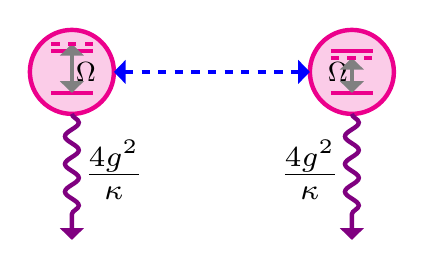
\begin{tikzpicture}[x=0.7in,y=0.7in]
\filldraw[color= magenta!100, fill=magenta!20, ultra thick](-.6,-1) circle (.3);
\filldraw[color=magenta!100, fill=magenta!20, ultra thick](1.4,-1) circle (.3);
\draw[color= magenta!100 , ultra thick] (-.45,-1.15)--(-0.75,-1.15);
\draw[color= magenta!100 , ultra thick] (-.45,-.85)--(-0.75,-0.85);
\draw[color= magenta!100 , ultra thick] (1.25,-1.15)--(1.55,-1.15);
\draw[color= magenta!100 , ultra thick] (1.25,-.85)--(1.55,-0.85);
\draw[blue , ultra thick , dashed , tipA-tipA] (-.3, -1.0) --(1.1,-1.0);
%\draw[orange , ultra thick , dashed , tipA-] (-.3, -1.15) --(1.1,-1.15);
\draw[violet , ultra thick , -tipA , decorate , decoration={snake,post length=1.65mm}] (-.6, -1.3) --(-.6,-2.2);
\draw[violet , ultra thick , -tipA , decorate , decoration={snake,post length=1.65mm}] (1.4, -1.3) --(1.4,-2.2);
\node at (-0.5,-1.0) {\scalebox{1.0}{$\Omega$}} ;
\node at (1.3,-1.0) {\scalebox{1.0}{$\Omega$}} ;
%\node at (-0.97,-0.85) {\scalebox{1.0}{$+\delta$}} ;
%\node at (1.77,-0.85) {\scalebox{1.0}{$-\delta$}} ;
\draw [gray, ultra thick , tipA-tipA] (-0.6,-1.15)--(-0.6,-.8);
\draw [gray, ultra thick , tipA-tipA] (1.4,-1.15)--(1.4,-.9);
\draw [dashed,color= magenta!100 , ultra thick] (1.25,-.90)--(1.55,-0.90);
\draw [dashed,color= magenta!100 , ultra thick] (-.45,-.80)--(-0.75,-0.80);
%\node at (0.4,-.7) {\scalebox{1.5}{$\frac{4 g^2 }{\kappa}$}} ;
\node at (-0.3,-1.7) {\scalebox{1.5}{$\frac{4 g^2}{\kappa}$}} ;
\node at (1.1,-1.7) {\scalebox{1.5}{$\frac{4 g^2}{\kappa}$}} ;
\end{tikzpicture}
}
\hspace*{.3in}
\subfigure[]{
\raisebox{-2cm}{
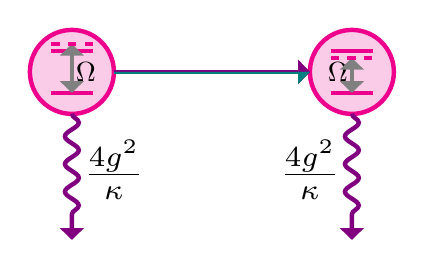
\begin{tikzpicture}[x=0.7in,y=0.7in]
\filldraw[color= magenta!100, fill=magenta!20, ultra thick](-.6,-1) circle (.3);
\filldraw[color=magenta!100, fill=magenta!20, ultra thick](1.4,-1) circle (.3);
\draw[color= magenta!100 , ultra thick] (-.45,-1.15)--(-0.75,-1.15);
\draw[color= magenta!100 , ultra thick] (-.45,-.85)--(-0.75,-0.85);
\draw[color= magenta!100 , ultra thick] (1.25,-1.15)--(1.55,-1.15);
\draw[color= magenta!100 , ultra thick] (1.25,-.85)--(1.55,-0.85);
\draw[ violet , ultra thick  , -tipA] (-.3, -1.0) --(1.1,-1.0);
%\draw[orange , ultra thick , dashed , tipA-] (-.3, -1.15) --(1.1,-1.15);
\draw[violet , ultra thick , -tipA , decorate , decoration={snake,post length=1.65mm}] (-.6, -1.3) --(-.6,-2.2);
\draw[violet , ultra thick , -tipA , decorate , decoration={snake,post length=1.65mm}] (1.4, -1.3) --(1.4,-2.2);
   \def\mypath{ (-.3, -1.0) --(1.1,-1.0)}
    \draw[color=violet ,  ultra thick , -tipA] \mypath;
    \begin{scope}[overlay]
      \clip (-1, -1) -- \mypath -- ++(1, 0) -- ++(0, -2) -- cycle;
      \draw[color=teal, -tipA , ultra thick] \mypath;
    \end{scope}
\node at (-0.5,-1.0) {\scalebox{1.0}{$\Omega$}} ;
\node at (1.3,-1.0) {\scalebox{1.0}{$\Omega$}} ;
%\node at (-0.97,-0.85) {\scalebox{1.0}{$+\delta$}} ;
%\node at (1.77,-0.85) {\scalebox{1.0}{$-\delta$}} ;
\draw [gray, ultra thick , tipA-tipA] (-0.6,-1.15)--(-0.6,-.8);
\draw [gray, ultra thick , tipA-tipA] (1.4,-1.15)--(1.4,-.9);
\draw [dashed,color= magenta!100 , ultra thick] (1.25,-.90)--(1.55,-0.90);
\draw [dashed,color= magenta!100 , ultra thick] (-.45,-.80)--(-0.75,-0.80);
%\node at (0.4,-.7) {\scalebox{1.5}{$\frac{8\left| g_1 \right| \left| g_2 \right|}{\kappa}$}} ;
\node at (-0.3,-1.7) {\scalebox{1.5}{$\frac{4 g^2}{\kappa}$}} ;
\node at (1.1,-1.7) {\scalebox{1.5}{$\frac{4 g^2}{\kappa}$}} ;
\end{tikzpicture}
}
}



\caption{(a) Symmetric dissipative interaction. 

(b) Uni-direction interaction do to inference of dissipative interaction and qubit-qubit couplings.   }

\end{figure}
\end{frame}

\begin{frame}
\frametitle{ Bell State Stabilization (Chiral Case)}
\centering
  $ |\Phi \rangle \propto |gg\rangle + \alpha | S \rangle  \quad H_S'| \Phi \rangle = 0 \Longrightarrow \alpha = \frac{\sqrt{2}\Omega}{2 \delta + i \Gamma}$
  
\vspace{3mm}

$\delta_1 = -\delta_2 = \delta$

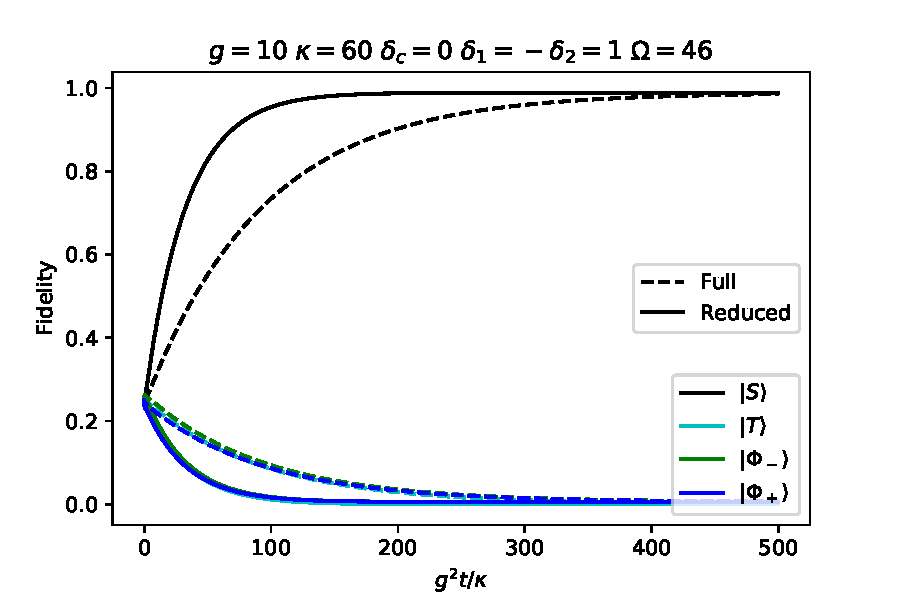
\includegraphics[scale=.6]{Asym_stabilization.pdf}

\end{frame}

\begin{frame}
\frametitle{Symmetric vs. Chiral}
\centering 
Ratio of respective performance metrics $R = \frac{M_{chiral}}{M_{sym}}$

\vspace{3mm}

$g = 10 \; \kappa = 60 \; \delta_1 = - \delta_2 = 1 \; \Omega=46$

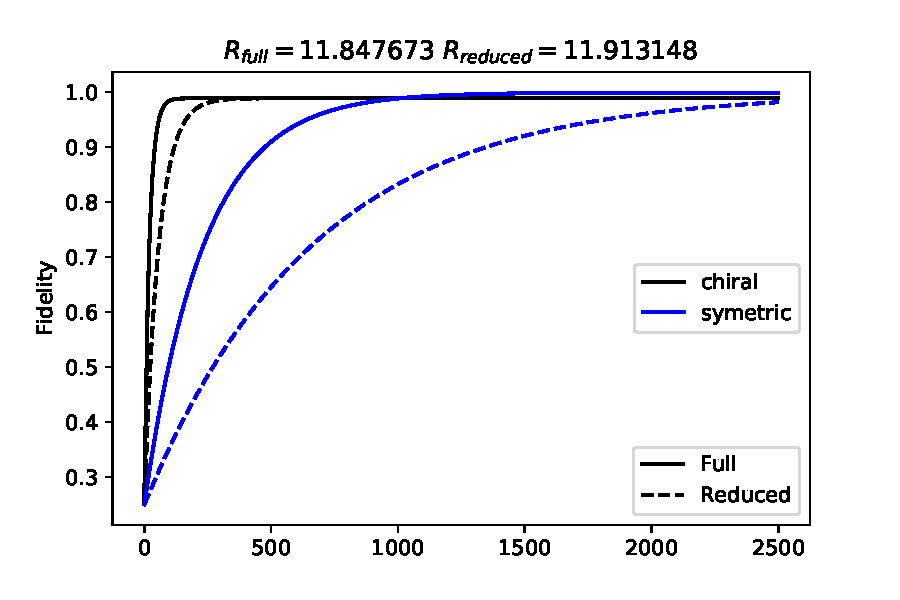
\includegraphics[scale=.6]{Sym_v_Chiral.pdf}

\end{frame}



\begin{frame}
\frametitle{Four-Qubit Entanglement }
\
$H_{SR} = g b^\dagger ( \sigma_1 + \sigma_2 + \sigma_3 + \sigma_4 ) + h.c.$

\begin{figure} \label{Fig:Detuning Pattern}
    \centering
     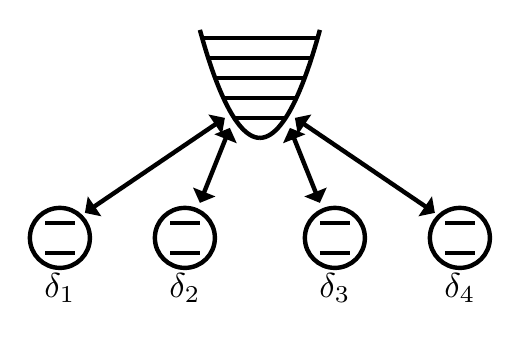
\begin{tikzpicture}[x=0.5in,y=0.5in]
    \draw[color=black!100 , ultra thick] (0,0) parabola (0.6,1.08) ;
    \draw[color=black!100 , ultra thick] (0.0,0.0) parabola (-0.6,1.08) ;
    \draw[color=black!100 , ultra thick] (-0.36514837167011072,.4) -- (0.36514837167011072,.4);
    \draw[color=black!100 , ultra thick] (0.2581988897471611,.2) -- (-0.2581988897471611,.2);
    \draw[color=black!100 , ultra thick] (0.44721359549995793,.6) -- (-0.44721359549995793,.6);
    \draw[color=black!100 , ultra thick] (0.5163977794943222,.8) -- (-0.5163977794943222,.8);
    \draw[color=black!100 , ultra thick] (0.57735026918962573,1.0) -- (-0.57735026918962573,1.0);
    \draw[color=black!100, ultra thick](-.75,-1) circle (.3);
    \node at (-.75 , -1.5){\scalebox{1.25}{$\delta_2$}} ;
    \draw[color=black!100, ultra thick](.75,-1) circle (.3);
    \node at (.75 , -1.5){\scalebox{1.25}{$\delta_{3}$}} ;
   % \draw[dotted , ultra thick] (.25,-1) -- (-.25,-1);
    \draw[color= black!100 , ultra thick] (-.6,-1.15)--(-0.9,-1.15);
    \draw[color= black!100 , ultra thick] (-.6,-.85)--(-0.9,-0.85);
    \draw[color= black!100 , ultra thick] (.6,-1.15)--(0.9,-1.15);
    \draw[color= black!100 , ultra thick] (.6,-.85)--(0.9,-0.85);
    \draw[color= black!100 , ultra thick] (-1.85,-1.15)--(-2.15,-1.15);
    \draw[color= black!100 , ultra thick] (-1.85,-.85)--(-2.15,-0.85);
    \draw[color= black!100 , ultra thick] (1.85,-1.15)--(2.15,-1.15);
    \draw[color= black!100 , ultra thick] (1.85,-.85)--(2.15,-0.85);
    \draw[color=black!100, ultra thick](-2,-1) circle (.3);
    \node at (-2.0 , -1.5){\scalebox{1.25}{$\delta_1$}} ;
    \draw[color=black!100, ultra thick](2,-1) circle (.3);
    \node at (2.0 , -1.5){\scalebox{1.25}{$\delta_{4}$}} ;
    \draw[black, ultra thick , tipA-tipA] (-0.6,-.65) -- (-0.3,0.1);
    \draw[black, ultra thick , tipA-tipA] (0.6,-.65) -- (0.3,0.1);
    \draw[black, ultra thick , tipA-tipA] (1.75,-.75) -- (0.35,0.2);
    \draw[black, ultra thick , tipA-tipA] (-1.75,-.75) -- (-0.35,0.2);
    \end{tikzpicture}
    
    \caption{Four qubits coupled to a mutual resonator mode with an associated detuning pattern $\Delta = ( \delta_1 , \delta_2 , \delta_3 , \delta_4)$. }
\end{figure}
\centering

``Engineered" jump operator is $\hat{S} =\sum_{i=1}^4 \sigma_i$.

\vspace{3mm}

$\dot{\rho}_S =  - \frac{i}{\hbar} [H_S, \rho] + \Gamma \mathcal{D}[\hat{S} ];\qquad \Gamma = \frac{4g^2}{\kappa}$


\end{frame}

\begin{frame}
\frametitle{Four-Qubit Entanglement: Symmetric vs. Chiral}
\begin{columns}
\begin{column}{0.47\textwidth}
$H_S =\underbrace{\sum_n \left( \frac{\delta_i}{2} \sigma_{zi} + \frac{\Omega}{2} \sigma_{xi} \right)}_{=H_{sym}}$

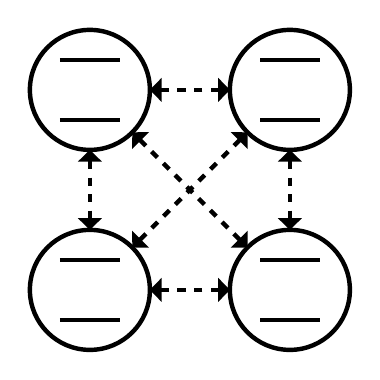
\begin{tikzpicture}[x=1.0in,y=1.0in]
\draw[color=black!100, ultra thick](.5,.5) circle (.3);
\draw[color=black!100, ultra thick](.5,-.5) circle (.3);
\draw[color=black!100, ultra thick](-.5,.5) circle (.3);
\draw[color=black!100, ultra thick](-.5,-.5) circle (.3);
\draw[dashed , ultra thick , tipA-tipA] (.2,.5) -- (-.2,.5);
\draw[dashed , ultra thick , tipA-tipA] (.2,-.5) -- (-.2,-.5);
\draw[dashed , ultra thick , tipA-tipA] (.5,.2) -- (.5,-.2);
\draw[dashed , ultra thick , tipA-tipA] (-.5,.2) -- (-.5,-.2);
\draw[color= black!100 , ultra thick] (.65,.35)--(.35,.35);
\draw[color= black!100 , ultra thick] (.65,.65)--(.35,.65);
\draw[color= black!100 , ultra thick] (-.65,.35)--(-.35,.35);
\draw[color= black!100 , ultra thick] (-.65,.65)--(-.35,.65);
\draw[color= black!100 , ultra thick] (.65,-.35)--(.35,-.35);
\draw[color= black!100 , ultra thick] (.65,-.65)--(.35,-.65);
\draw[color= black!100 , ultra thick] (-.65,-.35)--(-.35,-.35);
\draw[color= black!100 , ultra thick] (-.65,-.65)--(-.35,-.65);
\draw[dashed , ultra thick , tipA-tipA] (-.2878679656440358,-.2878679656440358)--(.2878679656440358,.2878679656440358);
\draw[dashed , ultra thick , tipA-tipA] (.2878679656440358,-.2878679656440358)--(-.2878679656440358,.2878679656440358);
\end{tikzpicture}
\end{column}

\begin{column}{0.47\textwidth}
$H_S = H_{sym} + \mathlarger{ \frac{i \Gamma}{2} \sum_{l > j}} \left( \sigma_l^\dagger \sigma_j - \sigma_l \sigma_j^\dagger \right) $

\vspace{3mm}

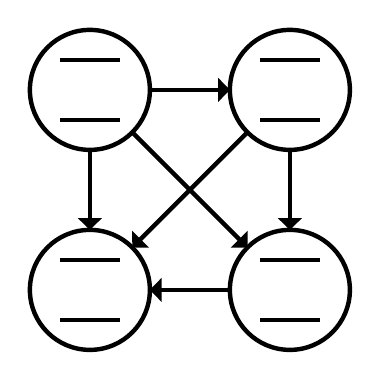
\begin{tikzpicture}[x=1.0in,y=1.0in]


\draw[color=black!100, ultra thick](.5,.5) circle (.3);
\draw[color=black!100, ultra thick](.5,-.5) circle (.3);
\draw[color=black!100, ultra thick](-.5,.5) circle (.3);
\draw[color=black!100, ultra thick](-.5,-.5) circle (.3);
\draw[ ultra thick , tipA-] (.2,.5) -- (-.2,.5);
\draw[ ultra thick , -tipA] (.2,-.5) -- (-.2,-.5);
\draw[ ultra thick , -tipA] (.5,.2) -- (.5,-.2);
\draw[ ultra thick , -tipA] (-.5,.2) -- (-.5,-.2);
\draw[color= black!100 , ultra thick] (.65,.35)--(.35,.35);
\draw[color= black!100 , ultra thick] (.65,.65)--(.35,.65);
\draw[color= black!100 , ultra thick] (-.65,.35)--(-.35,.35);
\draw[color= black!100 , ultra thick] (-.65,.65)--(-.35,.65);
\draw[color= black!100 , ultra thick] (.65,-.35)--(.35,-.35);
\draw[color= black!100 , ultra thick] (.65,-.65)--(.35,-.65);
\draw[color= black!100 , ultra thick] (-.65,-.35)--(-.35,-.35);
\draw[color= black!100 , ultra thick] (-.65,-.65)--(-.35,-.65);
\draw[ ultra thick , tipA-] (-.2878679656440358,-.2878679656440358)--(.2878679656440358,.2878679656440358);
\draw[ ultra thick , tipA-] (.2878679656440358,-.2878679656440358)--(-.2878679656440358,.2878679656440358);
\end{tikzpicture}
\end{column}
\end{columns}
\end{frame}

\begin{frame}
\frametitle{Entanglement Identification}
We define the purity of the density matrix : $tr ( \rho^2 ) $. 
 \centering
 \begin{eqnarray}
 tr( \rho^2 ) & = & 1 \quad\text{ for a pure state} \nonumber \\
  tr( \rho^2 ) & < & 1 \quad\text{ for a mixed state} \nonumber
 \end{eqnarray}
 
 Suppose I have an entangled state $|\Phi \rangle$ between two subsystems. Then by definition 
 \begin{equation}
 |\Phi \rangle \neq |\phi_1 \rangle \otimes |\phi_2 \rangle.
 \end{equation}
 When I trace over one  of the subsystem the result is not a pure state so the purity has to be less than one.
\end{frame}

\begin{frame}
\frametitle{Alternating Detunings: Symmetric \hspace{.5in} $\textcolor{blue}{\delta_a \; - \delta_a}$  $\textcolor{red}{\delta_b \;  - \delta_b}$}

Two qubit entanglement

\centering
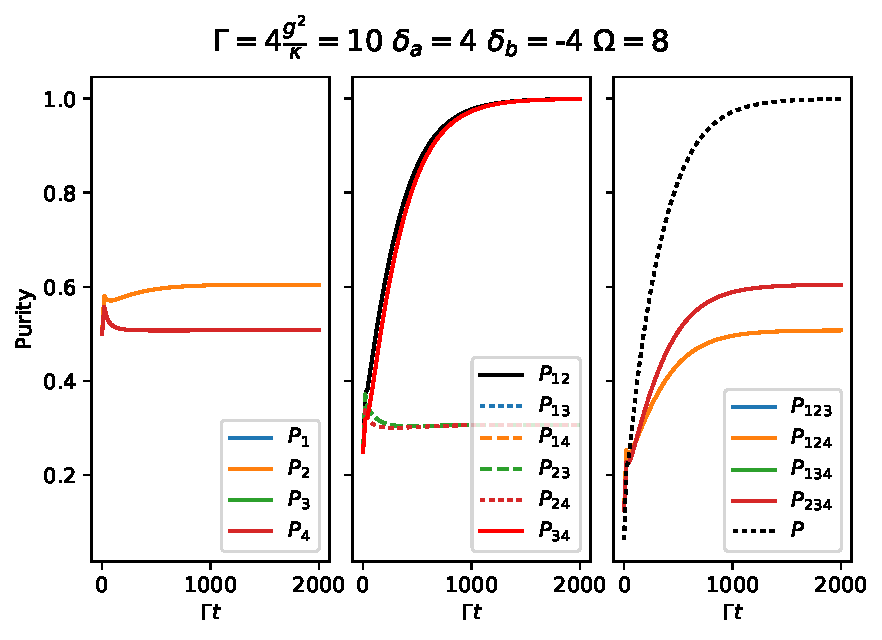
\includegraphics[scale=0.7]{Sym_Alter.pdf}
\end{frame}

\begin{frame}
\frametitle{Alternating Detunings: Chiral \hspace{.5in} $\textcolor{blue}{\delta_a \; - \delta_a}$  $\textcolor{red}{\delta_b \;  - \delta_b}$}

Two qubit entanglement

\centering 
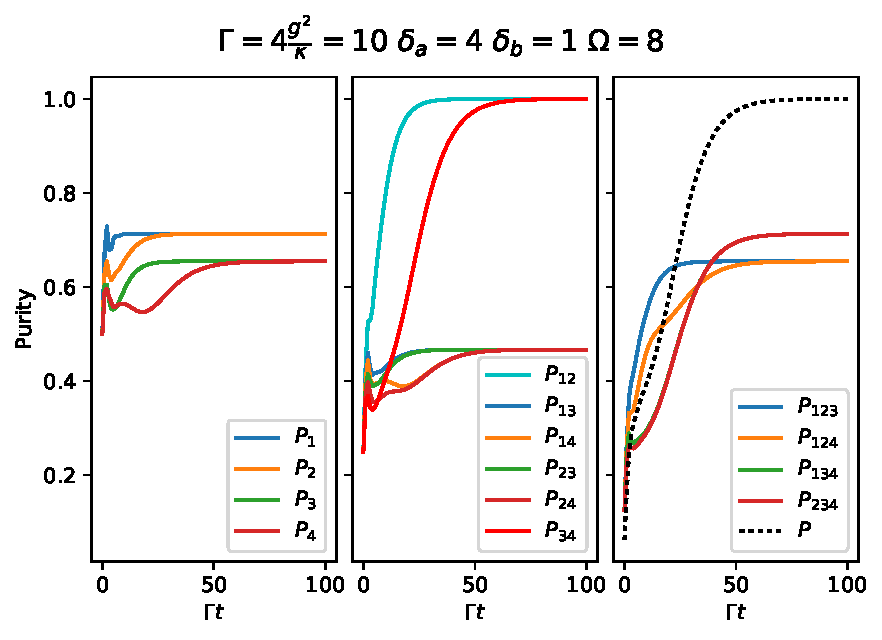
\includegraphics[scale=.70]{Chiral_Alternating.pdf}
\end{frame}

\begin{frame}
\frametitle{Staggered Detunings: Symmetric \hspace{.5in} $\textcolor{blue}{\delta_a}$ $\textcolor{red}{\delta_b}$ $\textcolor{blue}{-\delta_a}$ $\textcolor{red}{-\delta_b}$}


Non-local two qubit entanglement

\centering

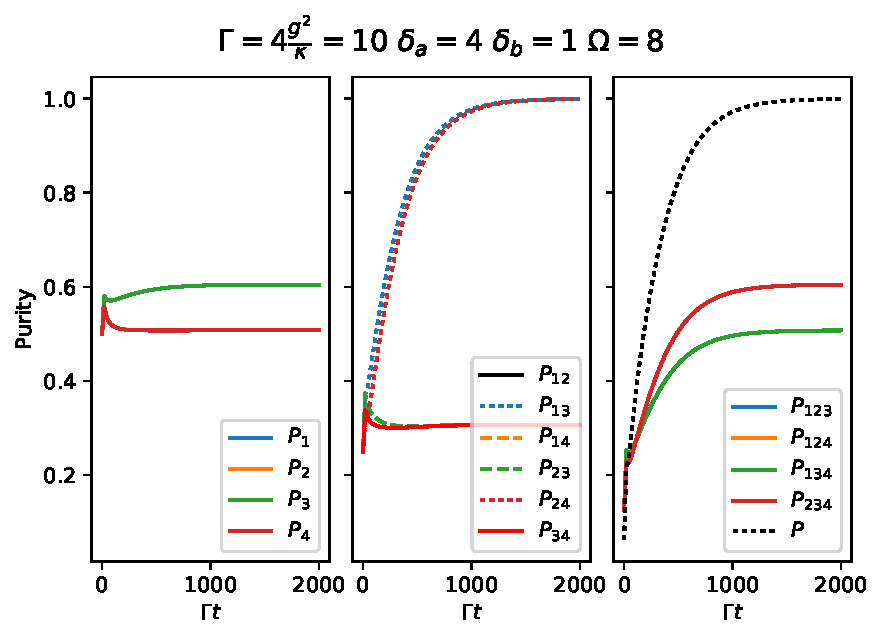
\includegraphics[scale=.7]{Sym_Stag.pdf}
\end{frame}

\begin{frame}
\frametitle{Staggered Detunings: Chiral \hspace{.5in} $\textcolor{blue}{\delta_a}$ $\textcolor{red}{\delta_b}$ $\textcolor{blue}{-\delta_a}$ $\textcolor{red}{-\delta_b}$}

Four-way entanglement: \textbf{Tetramer}

\centering

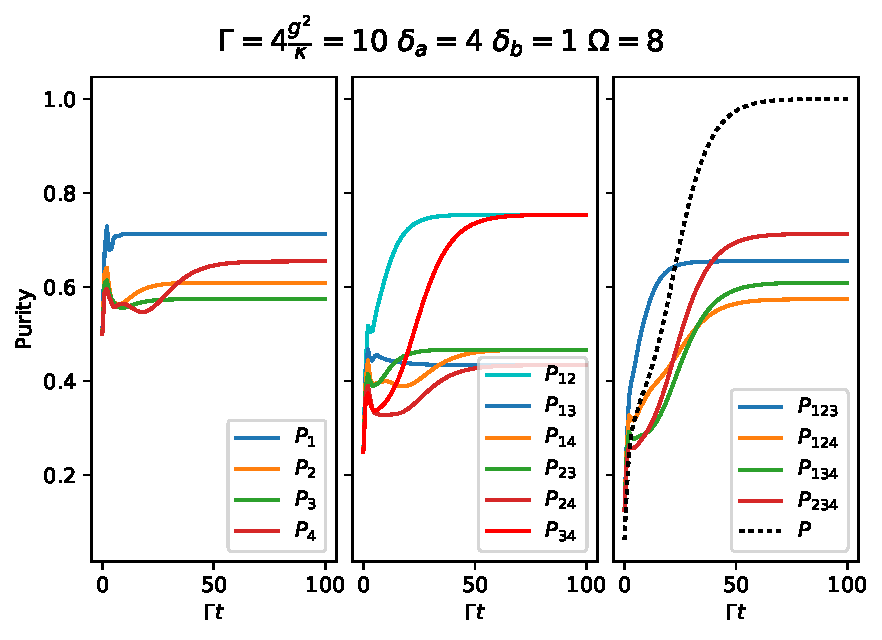
\includegraphics[scale=0.7]{Chiral_Stag.pdf}
\end{frame}


\begin{frame}
\frametitle{Caveat: four-qubit entanglement in symmetric case?}

Homogeneous detunings ($\textcolor{blue}{\delta \; \delta \; -\delta \; - \delta}$) \\+ pure initial state preparation, $\rho_S(0) = | gggg \rangle \langle gggg | $


 \begin{table}\label{Bell State Table}
\begin{tabular}{c|c}
Detuning Pattern & Stabilized State \\
\hline
$( \delta , - \delta , \delta , - \delta  )$ & $| S \rangle_{12} | S \rangle_{34} - | S \rangle_{14} | S \rangle_{23}.$  \\
$( \delta , - \delta , -\delta ,  \delta  )$ & $ | S \rangle_{12} | S \rangle_{34} + | S \rangle_{13} | S \rangle_{24}$  \\
$( \delta , \delta , - \delta , - \delta  )$  & $ | S \rangle_{13} | S \rangle_{24} + | S \rangle_{14} | S \rangle_{23}$ 
\end{tabular}
\caption{Table of detuning patterns and stabilized tetramer (four-way entangled state).}
\end{table}
\end{frame}

\begin{frame}
\frametitle{Example: Stabilization of  $| S \rangle_{13} | S \rangle_{24} + | S \rangle_{14} | S \rangle_{23}$}

\centering
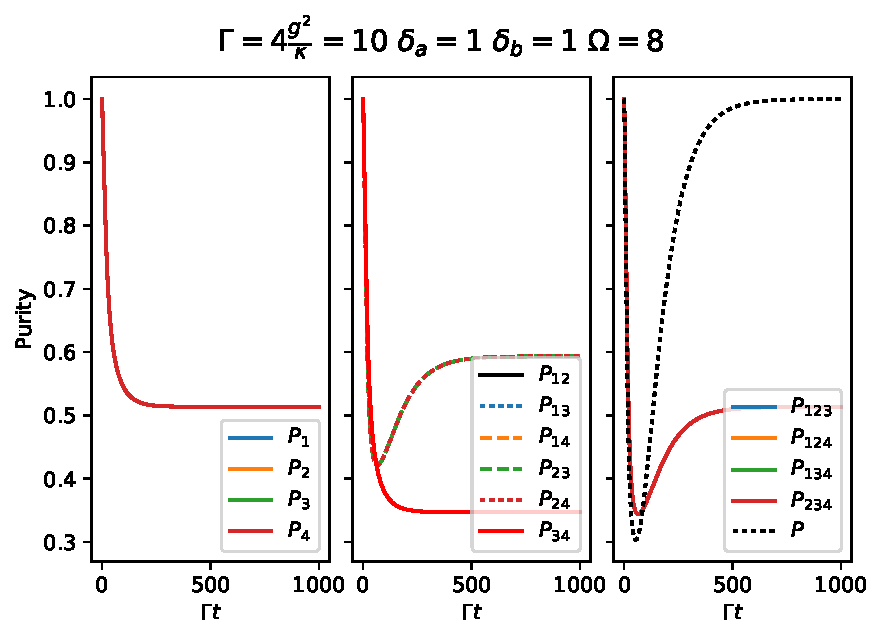
\includegraphics[scale=0.6]{Sym_Homo.pdf}



\end{frame}

\begin{frame}
\frametitle{Conclusions}
\begin{itemize}
\item Don't hide from dissipation, use it!
\item Adibatic elimination provides a way to identify engineered collapse operators
\item Chirality improves performance metric (fidelity $\times$ rate of Bell state stabilization) by 10x 
\item ``Engineered" dissipation can be used to stabilize four-qubit entanglement.
\begin{itemize}
\item The time scale and dynamics is different with and without chirality
\item Chirality is essential to purify mixtures into genuine multipartite entangled states
\end{itemize}
\end{itemize}
\end{frame}

\begin{frame}
\centering
\Huge Thank you!
\end{frame}

\end{document}